\section{Materiais,métodos e execução}

\subsection{Intel RAPL}
\begin{frame}{Intel RAPL}
    \begin{itemize}
        \item Otimizar o gerenciamento energético dos processadores Intel
        \item Monitoramento de alguns parametros como temperatura, potência e consumo energético
        \item Foi implementado a nível de hardware a partir da 6ª geração dos processadores Intel
        \item Segundo Khan at al 2018 \cite{khan2018IntelRapl}, a precisão do RAPL é bastante promisora e os valores reportados são precisos suficientemente para prever e modelar sistemas.
    \end{itemize}
\end{frame}

\begin{frame}{RAPL Power Domain}
    \begin{figure}
        \centering
        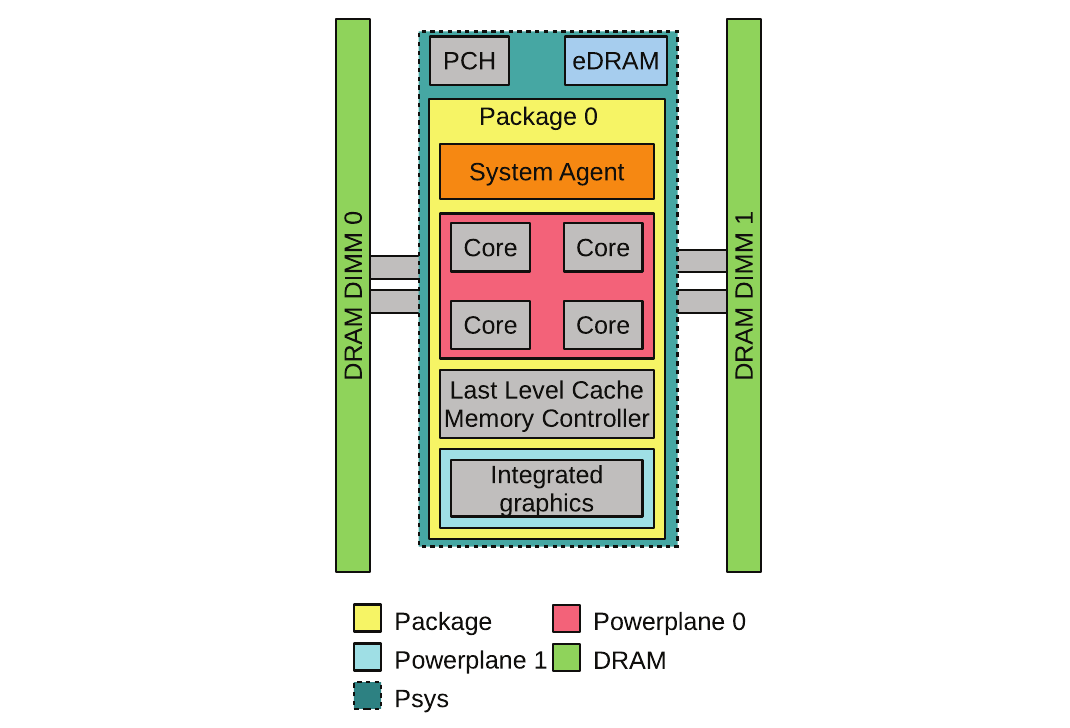
\includegraphics[width=0.61\linewidth]{images/powerDomainsRAPL.png}
        \caption{Intel RAPL Power Domains. Fonte: Khan at al 2018 \cite{khan2018IntelRapl}}
        \label{fig:powerDomains}
    \end{figure}
\end{frame}

\begin{frame}{Contadores de energia e limitações}
    \begin{itemize}
        \item Model-Specific Registers (MSRs) são registradores
        que fornecem acesso a diversas características e funcionalidades nos processadores x86
        \item MSR\_RAPL\_POWER\_UNIT de 32 bits sem sinal (0 a 4,294,967,295) 
        \item O registrador começa a contar a partir da inicialização do computador
        \item Quando este valor limite é atingido, o valor do registrador é reinicializado para 0 novamente.
        \item É de grande importância considerar a reinicialização
        dos registradores para não obter dados incorretos durante os experimentos
    \end{itemize}
\end{frame}

\subsection{Utilitários Linux}
\begin{frame}{Power Capping Framework}
    \begin{itemize}
        \item Ferramenta integrada ao Kernel Linux
        \item Permite expor informações de energia via \emph{sysfs} exportando informações sistemas de arquivos
        \item O framework cria de forma automática, uma árvore de diretórios com
        diversos objetos referente a interface de energia utilizada (The Linux Kernel Archives, 2024).
    \end{itemize}
\end{frame}

\begin{frame}{Árvore de Diretórios Power Capping Framework}
    \begin{figure}
        \centering
        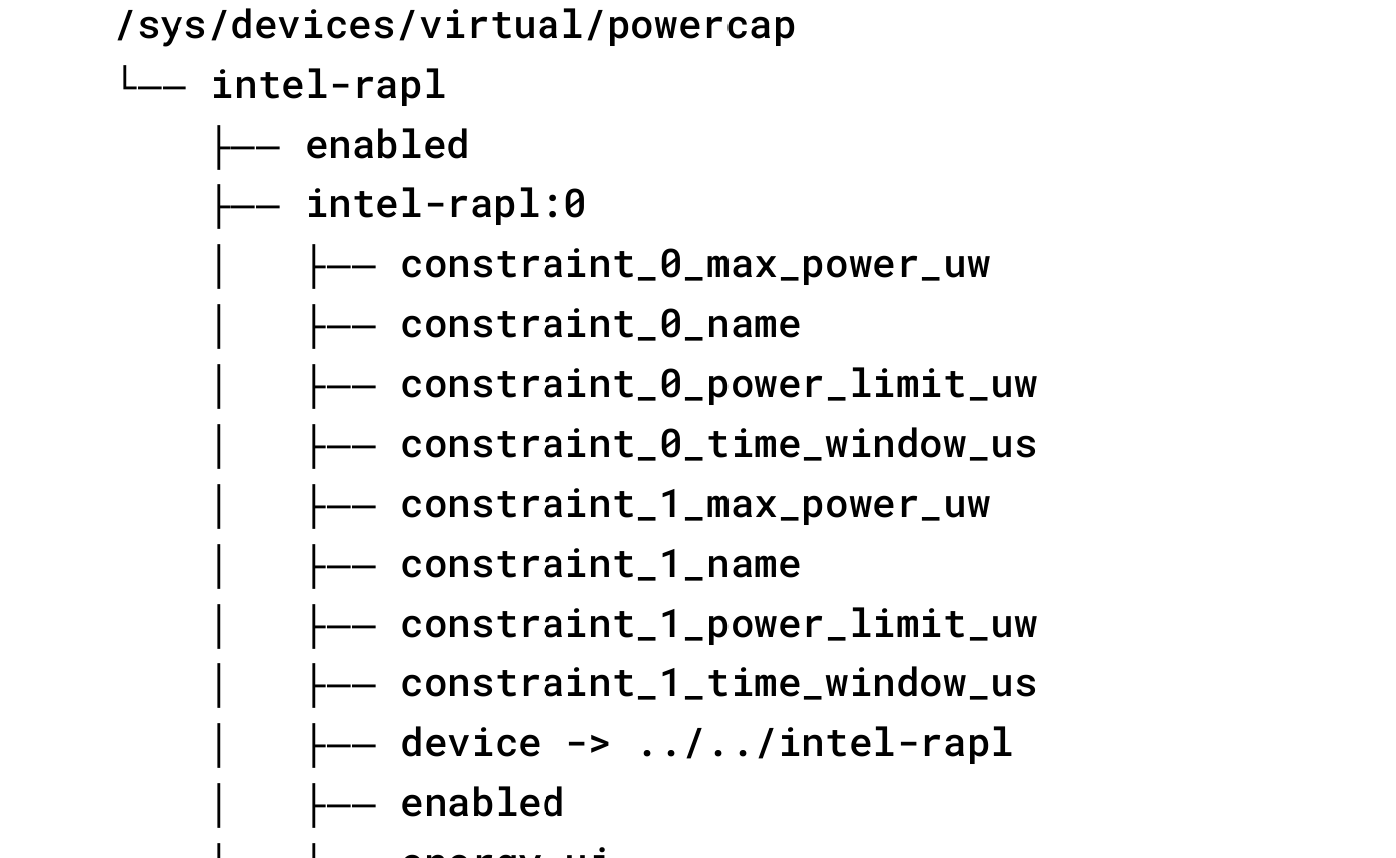
\includegraphics[width=0.65\linewidth]{images/powercap-tree.png}
        \caption{Árvore de Diretórios Power Capping Framework}
        \label{fig:powercap-tree}
    \end{figure}
\end{frame}

\begin{frame}{Shell}
    \begin{itemize}
        \item Interface entre o usuário e o sistema operacional
        \item O Shell é uma ferramenta essencial quando o foco é ter mais controle sobre o sistema operacional (RAYMOND, 2003)
        \item Funciona como um intermediário entre usuário e SO
        \item Essa interação pode ocorrer de forma iterativa e não iterativa
    \end{itemize}
\end{frame}

\begin{frame}{Shell Script}
    \begin{itemize}
        \item É uma linguagem de script voltada para automatização de tarefas em sistemas operacionais, sendo ela interpretada por um interpretador Shell
        \item Permite realizar diversas tarefas executando apenas um arquivo de script
        \item O interpretador analisa linha por linha e executa os comandos encontrados de forma sequencial
        \item Bastante útil ao executar diversos comandos, assim como a possibilidade de realização de tarefas repetitivas e automáticas
    \end{itemize}
\end{frame}

\begin{frame}{Bash}
    \begin{itemize}
        \item Bash é um shell desenvolvido por Brian Fox no Projeto GNU
        \item Atualmente é o Shell padrão de diversas distribuições Linux, como Ubuntu, Debian e Manjaro.
    \end{itemize}
\end{frame}

\begin{frame}{GNU Time}
    \begin{itemize}
        \item Utilizada para medir tempo e recursos consumidos por uma aplicação durante sua execução
        \item Utilização é bastante simples, com opções salvar a saída dos resultados em arquivo de texto
    \end{itemize}
    
    \begin{center}
        \texttt{/usr/bin/time ./meu\_programa > output.txt}
    \end{center}
\end{frame}

\subsection{The Computer Language Benchmark Game}
\begin{frame}{The Computer Language Benchmark Game}
    \begin{itemize}
        \item É um projeto de software livre que fornece um repositório com uma variedade de algorítimos simples que podem ser implementados em diversas linguagens de programação
        \item Um web site que centraliza todos os dados sobre códigos fontes, execução de teste e resultados
        \item O projeto fornece, além do código fonte, informações sobre compilação e execução dos algorítimos
    \end{itemize}
\end{frame}
\begin{frame}{CLBG Benchmarks}
	\centering
	
	\label{tbl:clbg_benchmarks}
	\begin{table}[h]
        %\caption{CLBG Benchmarks}
        \begin{tabular}{l|l}
        \textbf{Benchmarks} & \textbf{Descrição}   \\
        \hline
		fannkuch-redux      & Acesso indexado a minúsculas sequências inteiras            \\
		\hline
        n-body              & Dupla precisão para cálculo de N-body                       \\
		\hline
        spectral-norm       & Autovalor usando o método da potência                       \\
		\hline
        pidigits            & Streaming de aritmética de precisão arbitrária             \\
		\hline
        regex-redux         & Combina DNA e substitui por padrões mágicos                 \\
		\hline
        fasta               & Gerar e escrever sequências aleatórias de DNA               \\
		\hline
        k-nucleotide        & Atualiza hashtable e sequências de k-nucleotídeos           \\
		\hline
        reverse-complement  & Complemento reverso de sequências de DNA                     \\
		\hline
        binary-trees        & Aloca e desaloca muitas árvores binárias                    \\
		\hline
        mandelbrot          & Gera um conjunto de Mandelbrot em arquivo de bitmap portátil \\
    \end{tabular}
	\end{table}
\end{frame}

\subsection{Linguagens de Programação}
\begin{frame}{Linguagens de Programação}
    \begin{table}[h]
        \centering
        \fontsize{6}{7}\selectfont
        \begin{tabular}{l|l|l}
            \textbf{Linguagem} & \textbf{Versão} & \textbf{Compilador Open Source (Ubuntu 22.04)}\\
            \hline
            Ada & 10.5.1 & GNAT GPL Compiler \\
            \hline
            C & 11.4.0 & GCC \\
            \hline
            C\# & 7.0.115 & Mono \\
            \hline
            C++ & 11.4.0 & GCC \\
            \hline
            Chapel & 1.29.0 & Chapel Compiler \\
            \hline
            Dart & 3.2.6 & Dart SDK \\
            \hline
            Erlang &  26.2.2 & Erlang OTP \\
            \hline
            F\# & 7.0.115 & F\# Compiler \\
            \hline
            Fortran & 11.4.0 & GFortran \\
            \hline
            Go & 1.18.1 & Go Compiler \\
            \hline
            Haskell & 8.8.4 & GHC Haskell Compiler \\
            \hline
            Java & 19.0.2 & OpenJDK \\
            \hline
            Javascript & 18.19.0 & V8 \\
            \hline
            Julia & 1.9.3 & Julia Compiler \\
            \hline
            Lua & 5.3.0 & LuaJIT \\
            \hline
            Ocaml & 4.13.1 & OCaml Compiler \\
            \hline
            Perl & 5.34.1 & Perl Compiler \\
            \hline
            Php & 8.2.15 & PHP Compiler \\
            \hline
            Python & 3.10.12 & Python Interpreter \\
            \hline
            Racket & 8.2.0 & Racket Compiler \\
            \hline
            Ruby & 3.0.2 & Ruby Compiler \\
            \hline
            Rust & 1.75.0 & Rustc Compiler \\
            \hline
            Swift & 5.9.0 & Swift Compiler \\
        \end{tabular}
    \end{table}
\end{frame}

\subsection{Ambiente de testes}
\begin{frame}{Hardware}
    \centering
    \begin{table}[h]
        %\caption{Processador}
        %\label{tbl:cpu_specs}
        \centering
        \begin{tabular}{l|l}
            \textbf{Especificação} & \textbf{Descrição} \\
            \toprule
            Modelo & Intel® Core™ i5-10210U \\
            \hline
            Geração & 10ª Geração \\
            \hline
            Codinome & Comet Lake \\
            \hline
            Nº de núcleos & 4 \\
            \hline
            Threads & 8 \\
            \hline
            Frequência base & 1.60 GHz \\
            \hline
            Frequência turbo max & 4.20 GHz \\
            \hline
            Cache & 6 MB Intel® Smart Cache \\
            \hline
            Litografia & 14 nm \\
            \hline
            TDP & 15 W \\
            \hline
        \end{tabular}
    \end{table}
\end{frame}

\begin{frame}{Hardware}
    \centering
    \begin{table}[h]
        %\caption{Armazenamento e energia}
        %\label{tbl:other_specs}
        \centering
        %\rowcolors{2}{lightgray!30}{white}
        \begin{tabular}{l|l}
            %\toprule
            \textbf{Especificação} & \textbf{Descrição} \\
            \toprule
            Memória DRAM & 8GB (Dual Channel) \\
            \hline
            Frequência da Memória DRAM & 2666MHz \\
            \hline
            Tipo de Memória DRAM & DDR4 \\
            \hline
            Armazenamento Interno & 256GB \\
            \hline
            Tipo do Armazenamento Interno & PCIe NVMe M.2\\
            \hline
            Potência Máxima da Fonte de Alimentação & 45W\\
            %\bottomrule
        \end{tabular}
    \end{table}
\end{frame}

\begin{frame}{Sistema Operacional}
    \centering
    \begin{table}[h]
        %\caption{Sistema Operacional}
        %\label{tbl:so_specs}
        \centering
        %\rowcolors{2}{lightgray!30}{white}
        \begin{tabular}{l|l}
            \textbf{Especificação} & \textbf{Descrição} \\
            \toprule
            Distribuição & Ubuntu \\
            \hline
            Versão & 22.04 LTS  \\
            \hline
            Codinome & Jammy Jellyfish \\
            \hline
            Ambiente de desktop & KDE Plasma \\
            \hline
            Kernel & Linux 5.15 \\
            \hline
            Arquitetura & x86 64 bits \\
            \hline
            Tipo de instalação & Desktop\\
            %\bottomrule
        \end{tabular}
    \end{table}
\end{frame}

